\documentclass[12pt]{article}
\usepackage{amsmath}
\usepackage{amssymb}
\usepackage{amsthm}
\usepackage{amsfonts}
\usepackage{graphicx} 
\usepackage{amsthm}
\graphicspath{{./images/}}

\title{Desmos \#5:
\\Using the Alternating Series
\\Estimation Theorem}
\author{Rafael Betita\\
MATH 005BH - Single Variable Calculus II}
\date{November 8, 2018}

\begin{document}
\maketitle
\newpage
\section{Review of Absolute \& Conditional\\ Convergence}
In sections 11.5 and 11.6, you learned about absolute and conditional convergence. So when we are looking at a series of the form $\sum_{n=1}^\infty(-1)^nb_n$ what is the first thing we consider? Briefly explain, when you look at this series, how you approach checking this series for convergence. What do you do first? Second?


\vspace{5mm}
\noindent Upon first glance, it is clear that the series can be considered as an alternating series. This means that each term alternates from negative to positive. It is appropriate to use the Alternating Series Test to test for convergence. This test postulates two conditions to be true:

\begin{enumerate}
    \item $\lim_{n\to\infty}b_n = 0$
    \item $\{b_n\}$ is decreasing
\end{enumerate}
\noindent If these two conditions are met, $\sum_{n=1}^\infty(-1)^nb_n$ must be convergent.

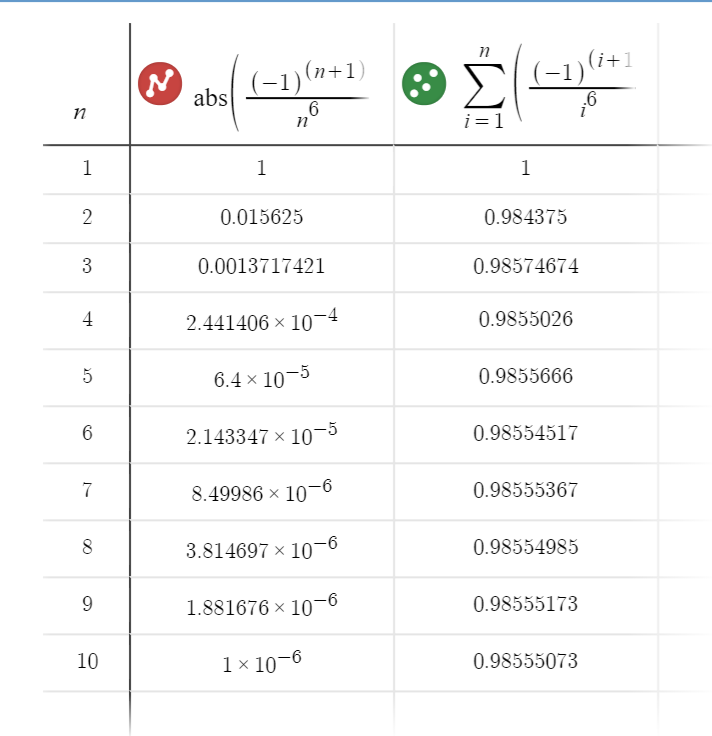
\includegraphics[width=\linewidth]{11_5_23}
We use $n=5$ for our sum, since $s_6$ is lower than the desired error bound
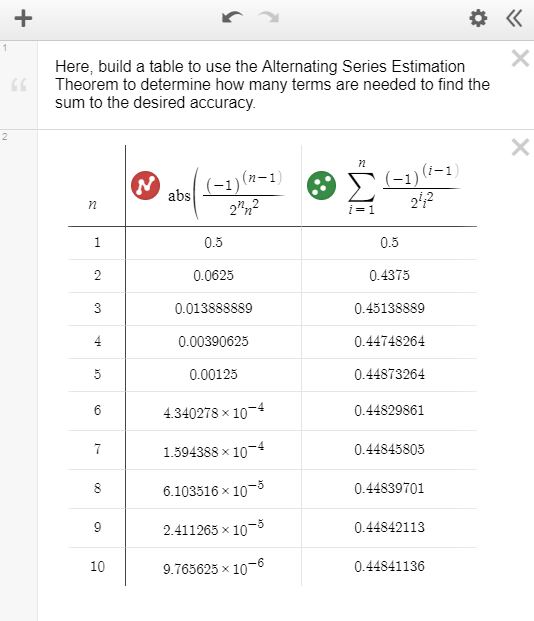
\includegraphics[width=\linewidth]{11_5_25}
We use $n=5$ for our sum, since $s_6$ is lower than the desired error bound 

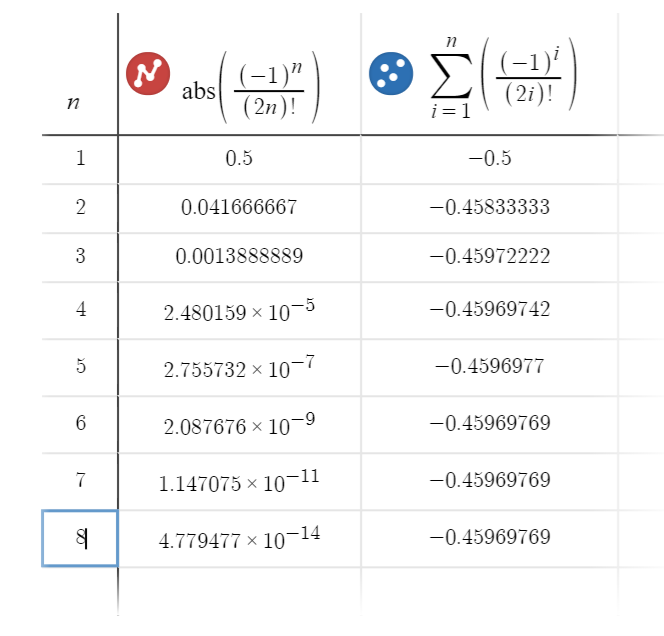
\includegraphics[width=\linewidth]{11_5_27}
$s_4$ does not affect the sum of $s_3$ so we can use $s_3$

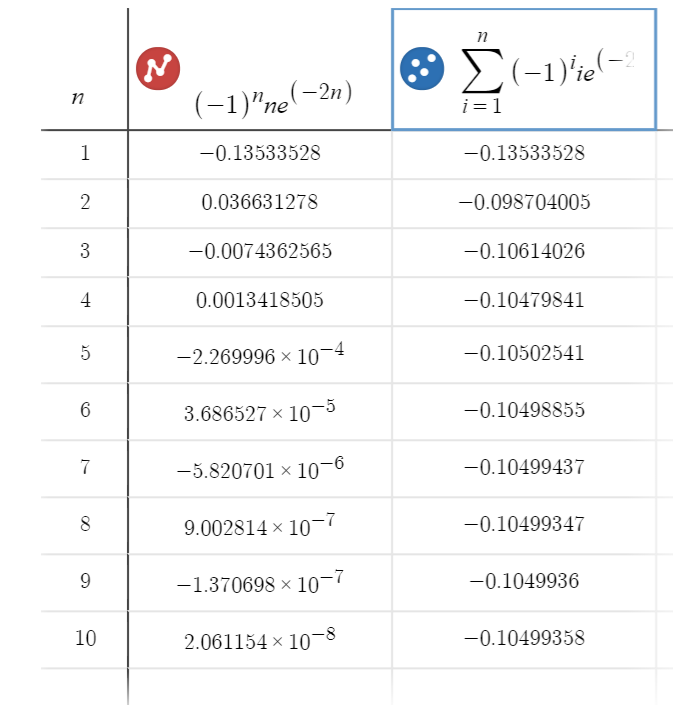
\includegraphics[width=\linewidth]{11_5_29}
$s_6$ does not affect the sum of $s_5$ so we can use $s_5$

\end{document}